\chapter*{Acknowledgements}
\addcontentsline{toc}{chapter}{Acknowledgements}

\section*{Institutions}

We thank Columbia University along with the Departments of
Statistics and Political Science, the Applied Statistics Center, the
Institute for Social and Economic Research and Policy ({\sc iserp}),
and the Core Research Computing Facility.

\section*{Grants and Corporate Support}

Without the following grant and consulting support, Stan would not exist.

\subsection*{Current Grants}

\begin{itemize}
\item
 U.~S.\ Department of Education Institute of Education Sciences
\begin{itemize}\small
\item Statistical and Research Methodology: Solving
Difficult Bayesian Computation Problems in Education Research Using Stan
\end{itemize}
\item  Alfred P.\ Sloan Foundation
\begin{itemize}\small
\item G-2015-13987: Stan Community and Continuity (non-research)
\end{itemize}
\item U.~S.\ Office of Naval Research (ONR)
\begin{itemize}\small
\item Informative Priors for Bayesian Inference and Regularization
\end{itemize}
\end{itemize}
%


\subsection*{Previous Grants}

Stan was supported in part by
%
\begin{itemize}
\item
U.~S.\ Department of Energy
\begin{itemize}\small
\item DE-SC0002099: Petascale Computing
\end{itemize}
%
\item
U.~S.\ National Science Foundation
\begin{itemize}\small
\item
ATM-0934516: Reconstructing Climate from Tree Ring Data
\item
CNS-1205516: Stan: Scalable Software for Bayesian Modeling
\end{itemize}
%
\item
U.~S.\ Department of Education Institute of Education Sciences
\begin{itemize}\small
\item ED-GRANTS-032309-005:
Practical Tools for Multilevel Hierarchical Modeling in Education
 Research
\item R305D090006-09A: Practical Solutions for Missing Data
\end{itemize}
\item
U.~S.\ National Institutes of Health
\begin{itemize}
\item 1G20RR030893-01: Research Facility Improvement Grant
\end{itemize}
\end{itemize}


\section*{Stan Logo}

The original Stan logo was designed by Michael Malecki.  The current
logo is designed by Michael Betancourt, with special thanks to
Stephanie Mannheim (\url{http://www.stephaniemannheim.com/}) for
critical refinements.  The Stan logo is copyright 2015 Michael
Betancourt and released for use under the CC-BY ND 4.0 license (i.e.,
no derivative works allowed).


\section*{Individuals}

We thank John Salvatier for pointing us to automatic differentiation
and \HMC in the first place.  And a special thanks to Kristen van
Leuven (formerly of Columbia's ISERP) for help preparing our initial
grant proposals.

\subsection*{Code  and Doc Patches}

Thanks for bug reports, code patches, pull requests, and diagnostics
to:
Ethan Adams,
Avraham Adler,
Jarret Barber,
David R.~Blair,
Miguel de Val-Borro,
Ross Boylan,
Eric N.~Brown,
Devin Caughey,
Emmanuel Charpentier,
Daniel Chen,
Jacob Egner,
Ashley Ford,
Jan Gl\"ascher,
Jan Gleixner,
Robert J.\ Goedman,
Danny Goldstein,
Tom Haber,
B.~Harris,
Kevin Van Horn,
Stephen Hoover,
Andrew Hunter,
Bobby Jacob,
Bruno Jacobs,
Filip Krynicki
Dan Lakeland,
Devin Leopold,
Nathanael I.~Lichti,
Jussi M\"a\"att\"a,
Titus van der Malsburg,
P.~D.~Metcalfe,
Kyle Meyer,
Linas Mockus,
Jeffrey Oldham,
Tomi Peltola,
Joerg Rings,
Cody T.\ Ross,
Patrick Snape,
Matthew Spencer,
Wiktor Soral,
Alexey Stukalov,
Fernando H.~Toledo,
Arseniy Tsipenyuk,
Zhenming Su,
Matius Simkovic,
Matthew Zeigenfuse,
and
Alex Zvoleff.

Thanks for documentation bug reports and patches to:
alvaro1101 (GitHub handle),
andrasm (GitHub handle),
Avraham Adler,
Chris Anderson,
Asim,
Jens Astrom,
Jarret Barber,
Ryan Batt,
Frederik Beaujean,
Guido Biele,
Luca Billi,
Chris Black,
botanize (GitHub handle),
Portia Brat,
Arthur Breitman,
Eric C.~Brown,
Eric N.~Brown,
Juan Sebasti\'an Casallas,
Alex Chase,
Daniel Chen,
Roman Cheplyaka,
Andy Choi,
David Chudzicki,
Michael Clerx,
Marco Colombo,
Luis Damiano,
Andria Dawson,
daydreamt (GitHub handle),
Conner DiPaolo,
Eric Innocents Eboulet,
Jos\'{e} Rojas Echenique,
Andrew Ellis,
G\"{o}k\c{c}en Eraslan,
Rick Farouni,
Avi Feller,
Seth Flaxman,
Wayne Folta,
Ashley Ford,
Kyle Foreman,
Mauricio Garnier-Villarreal,
Christopher Gandrud,
Jonathan Gilligan,
Aaron Goodman,
John Hall,
David Hallvig,
David Harris,
C. Hoeppler,
Cody James Horst,
Herra Huu,
Bobby Jacob,
Max Joseph,
Julian King,
Fr\"anzi Korner-Nievergelt,
Juho Kokkala,
Takahiro Kubo,
Mike Lawrence,
Louis Luangkesorn,
Tobias Madsen,
Stefano Mangiola,
David Manheim,
Stephen Martin,
Sean Matthews,
David Mawdsley,
Dieter Menne,
Evelyn Mitchell,
Javier Moreno,
Robert Myles,xs
Sunil Nandihalli,
Eric Novik,
Julia Palacios,
Tamas Papp,
Anders Gorm Pedersen,
Tomi Peltola,
Alex Perrone,
Andre Pfeuffer,
Sergio Polini,
Joerg Rings,
Sean O'Riordain,
Brendan Rocks,
David M.\ Rogers,
Cody Ross,
Mike Ross,
Tony Rossini,
Nathan Sanders,
Massimo Santini,
James Savage,
Terrance Savitsky,
Dan Schrage,
Gary Schulz,
seldomworks (GitHub handle),
Janne Sinkkonen,
skanskan (GitHub handle),
Yannick Spill,
Trey Spiller,
sskates (GitHub handle),
ssp3nc3r (GitHub handle),
Martin Stjernman,
Dan Stowell,
Alexey Stukalov,
Dougal Sutherland,
John Sutton,
Maciej Swat,
Jonathan Sweeney,
J.~Takoua,
Andrew J.~Tanentzap,
Shravan Vashisth,
Aki Vehtari,
Lukas Vermeer,
Damjan Vukcevic,
Matt Wand,
Amos Waterland,
Sebastian Weber,
Sam Weiss,
Lukasz Wiklendt,
wrobell (GitHub handle),
Howard Zail,
Jon Zelner, and
Xiubo Zhang

Thanks to Kevin van Horn for install instructions for Cygwin and to
Kyle Foreman for instructions on using the MKL compiler.


\subsection*{Bug Reports}

We're really thankful to everyone who's had the patience to try
to get Stan working and reported bugs.  All the gory details are
available from Stan's issue tracker at the following URL.
%
\begin{quote}
\url{https://github.com/stan-dev/stan/issues}
\end{quote}




\vfill
\begin{center}
\hfill
\begin{minipage}[b]{2in}
  \footnotesize {\it Stanislaw Ulam, namesake of Stan and co-inventor
    of Monte Carlo methods \citep{MetropolisUlam:1949}, shown here
    holding the Fermiac, Enrico Fermi's physical Monte Carlo simulator
    for neutron diffusion.}
  \\[3pt] \mbox{ } \hfill
  {\scriptsize Image from \citep{Giesler:2000}.}
\end{minipage} \ \ \ \ \
\begin{minipage}[b]{1.5in} \mbox{ } \hfill
  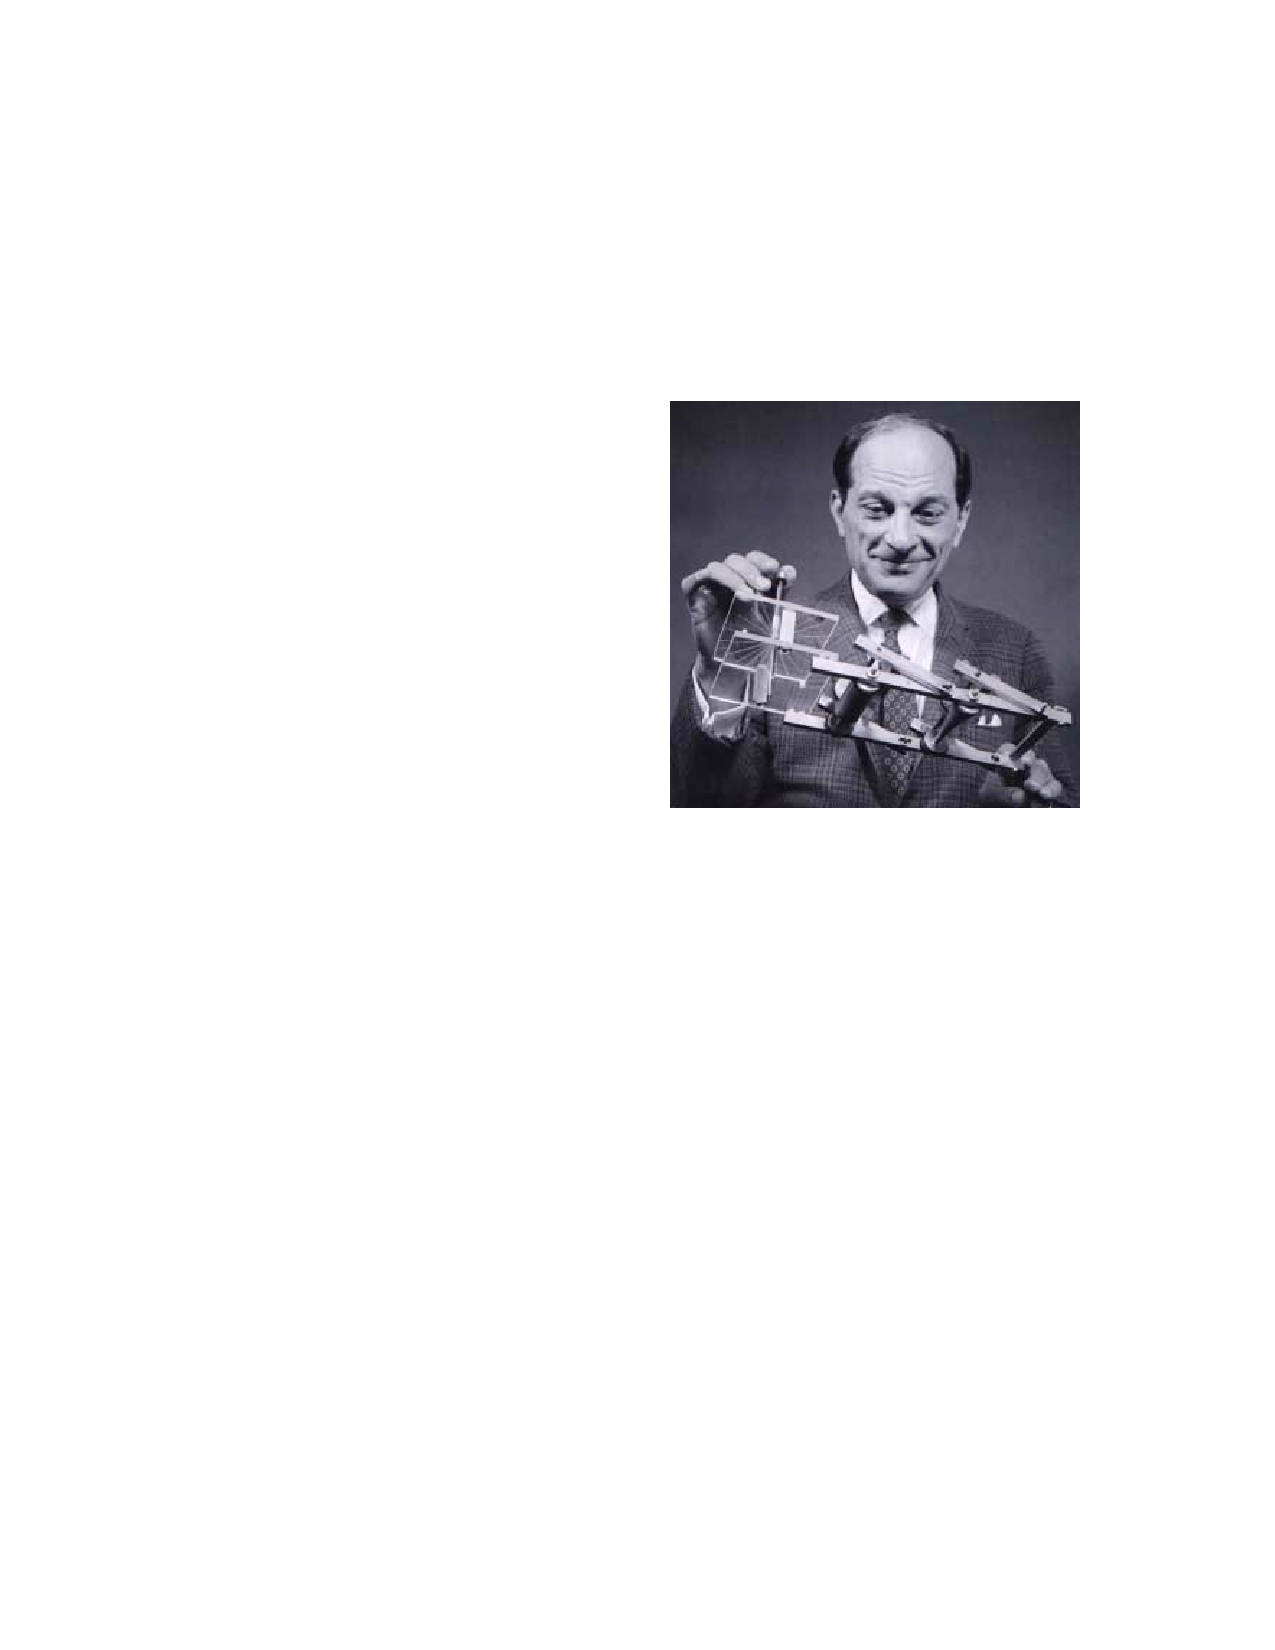
\includegraphics[width=1.5in]{img/ulam-fermiac.pdf}
\end{minipage}
\end{center}
